% Reproduction manuscript. Compile with pdflatex (twice for references).
% Upload manuscript.tex and figures/ to Overleaf, set compiler to pdfLaTeX.
\documentclass[11pt,a4paper]{article}

\usepackage[T1]{fontenc}
\usepackage[utf8]{inputenc}
\usepackage{lmodern}
\usepackage[margin=2.5cm]{geometry}
\usepackage{microtype}
\usepackage{amsmath,amssymb}
\usepackage{graphicx}
\usepackage{booktabs}
\usepackage{array}
\usepackage{caption}
\usepackage{enumitem}
\usepackage[hidelinks]{hyperref}

\captionsetup{font=small,labelfont=bf}
\setlist{itemsep=2pt,topsep=3pt}
\renewcommand{\arraystretch}{1.15}

\title{\vspace{-1.2cm}\bfseries A reproduction and analysis of a generative
transformer for spider silk protein design}
\author{}
\date{}

\begin{document}
\maketitle
\vspace{-1.0cm}

\begin{abstract}
\noindent
This report reproduces the generative modelling framework of Lu, Kaplan and
Buehler (\textit{Advanced Functional Materials}, 2024), which fine-tunes a
253.6 million parameter language model on major ampullate spidroin sequences to
predict fibre-level mechanical properties and to design sequences for target
properties. Using the authors' released checkpoint, we rebuilt the training
dataset and the normalisation constants from primary sources, verified the
architecture, and re-ran the reported design procedure. The dataset
reconstruction reaches the published count of 1{,}033 sequences exactly, and the
recovered normalisation constants match the published table on all eight
properties. Running the design procedure with the reported sampling budget, our
best selected candidate falls below the published coefficient of determination
($R^2$) on all eight property targets, with a mean shortfall of 0.27. When the
authors' own generated sequences are submitted to the forward task, the model
returns the published property vectors exactly on four of five sets, which
places the shortfall in the candidate search rather than in the model or its
evaluation. Four additional analyses characterise the fine-tuned model: the
reported $R^2$ grows steeply with the number of sampled candidates; deleting
mechanically relevant sequence motifs moves the forward prediction no more than
a length-matched control; the forward task returns the exact training label for
71\% of fine-tuning sequences; and prediction accuracy falls from
$R^2 = 0.83$ on the training family to between $-0.27$ and $-0.54$ on other
spidroin families. These observations are consistent with the model behaving
largely as a retrieval system over its fine-tuning set, which is the expected
consequence of training on all available data without a held-out split.
\end{abstract}

\section{Introduction}

Spider dragline silk combines high tensile strength with high extensibility,
giving it a toughness that exceeds most engineered fibres of comparable weight.
These properties arise from the sequence of the underlying proteins, called
spidroins, so a model that maps sequence to properties would support the design
of new fibres by selecting sequences. Lu, Kaplan and Buehler \cite{lu2024}
proposed such a model, named SilkomeGPT. It is a decoder-only transformer,
pretrained on a large set of protein sequences and fine-tuned on roughly one
thousand major ampullate spidroin (MaSp) sequences paired with measured
mechanical properties. The model is used in two directions: a forward task that
predicts eight property values from a sequence, and an inverse task that
generates a sequence for a requested set of eight values. The two are combined
in a cycle, and the agreement between the requested and the predicted
properties is reported as the coefficient of determination.

The aim of this work was to reproduce the reported results using the released
model and, where the paper leaves a choice unspecified, to measure the effect of
that choice rather than assume it away. A second aim was to characterise the
behaviour of the fine-tuned model using experiments that the original paper did
not report. All quantities stated below were produced by scripts in an
accompanying code repository, and each is recorded together with the software
versions, random seed and model revision that produced it.

\section{Background}

\subsection{Proteins, silk and the property vector}

A protein is a chain of amino acids, of which twenty are standard, so a protein
can be written as a string over a twenty-letter alphabet. Spidroins have a
characteristic layout in which two non-repetitive terminal domains flank a long
repetitive core. The core alternates poly-alanine runs, which pack into rigid
crystalline sheets and contribute strength and stiffness, with glycine-rich
motifs such as GGX and GPGXX, which are disordered and contribute extensibility.

The mechanical properties come from a single tensile test in which a fibre is
stretched until it breaks. Four quantities are read from the resulting
stress-strain curve: toughness (the energy absorbed per unit volume, the area
under the curve), elastic modulus (the initial slope), tensile strength (the
peak stress) and strain at break (the extension at failure). Each is measured
several times, so each has an associated standard deviation. The paper
concatenates the four properties and their four standard deviations into an
eight-dimensional vector,
\[
[\text{toughness},\ \text{SD},\ E,\ \text{SD},\ \text{strength},\ \text{SD},\
\text{strain},\ \text{SD}],
\]
and normalises every entry to the interval $[0,1]$ by min-max scaling. The
ordering is fixed and is not labelled in the model input, so the model learns
the positions.

The data come from the Silkome dataset \cite{arakawa2022}, which pairs spidroin
sequence records with mechanical measurements taken on the dragline fibre of
individual spiders. Because the mechanical test is performed on dragline, and
dragline is composed of MaSp, the properties in the dataset describe MaSp even
when a non-MaSp sequence from the same spider is present. This point is relevant
to the family-transfer analysis in Section~\ref{sec:nonmasp}.

\subsection{The model and its three tasks}

SilkomeGPT is a GPT-NeoX-style transformer with 12 layers, 8 attention heads, a
hidden dimension of 1024, a feed-forward width of 4096 and rotary positional
embeddings. Its tokeniser uses byte-pair encoding with a vocabulary of up to
50{,}000 tokens, which merges frequent adjacent pieces into single tokens. This
compresses the repetitive spidroin sequences substantially, so token counts are
smaller than residue counts and are not proportional to them.

Fine-tuning taught the model three text formats. The \texttt{Sequence} task is
plain next-token prediction. The \texttt{CalculateSilkContent} task, the forward
task, takes a sequence in angle brackets and produces the eight property values
in square brackets. The \texttt{GenerateSilkContent} task, the inverse task,
takes eight values and produces a sequence. The forward and inverse tasks carry
the same information in opposite directions, which is what allows the cycle
described below.

Training used all known sequence-property pairs, with no held-out test set. Any
accuracy measured on those pairs is therefore an in-sample measurement, which
bounds performance from above and does not separate a model that has learned the
mapping from one that has memorised the pairs.

\subsection{The coefficient of determination as the paper applies it}

For true values $y_i$ and predictions $\hat{y}_i$ with mean $\bar{y}$,
\[
R^2 = 1 - \frac{\sum_i (y_i - \hat{y}_i)^2}{\sum_i (y_i - \bar{y})^2}.
\]
A value of 1 is a perfect fit, 0 matches always predicting the mean, and
negative values are worse than predicting the mean. Negative values occur
frequently in the analyses below.

The paper computes $R^2$ across the eight entries of a single property vector:
for one designed sequence, its eight predicted values against the eight
requested values. This is a self-consistency measure of the forward and inverse
tasks, and the paper describes it as such. It is not a regression $R^2$ over a
set of held-out sequences, and the two are different quantities. Two consequences
follow. The denominator is the spread of the eight requested values, so a target
whose entries are tightly clustered gives a small denominator and a sensitive
$R^2$. Four of the eight entries are standard deviations, which vary less across
the dataset and are easier to predict, so an $R^2$ over all eight can be
respectable while the four mechanical entries are predicted poorly. This report
gives the four mechanical entries separately where that distinction matters.

\section{Methods}

\subsection{Model access and verification}

We used the released checkpoint \texttt{lamm-mit/SilkomeGPT} at a fixed
revision, loaded with half precision on a single laptop GPU (NVIDIA RTX 4050,
6~GB). The checkpoint requires custom model code executed at load time; the
resolved commit hash was recorded so that later runs use the same weights.

The loaded model reports 12 layers, 8 heads, hidden dimension 1024 and
feed-forward width 4096, matching the paper, and a parameter count of
253{,}556{,}736, which agrees with the stated 253.6 million. As a stronger check,
the paper prints one fine-tuning record in full, giving a sequence and the eight
values paired with it. Submitting that sequence to the forward task returns
$[0.327, 0.356, 0.261, 0.287, 0.437, 0.190, 0.220, 0.301]$, which is the
published vector on all eight entries. This exercises the tokeniser, the prompt
format, the weights and the output parser together against a known answer.

\subsection{Dataset reconstruction}
\label{sec:dataset}

The paper states that its dataset contains 1{,}033 pairs constructed from the
Silkome data, but does not give the construction rule, and the pairs are not in
the released repository. We rebuilt them from the Silkome release, which
provides a protein FASTA file of 11{,}155 records and a table of mechanical
properties for 446 individual spiders. Joining the two files on the individual
spider identifier, keeping rows with all eight mechanical values present, and
keeping records whose type label begins with ``MaSp'' yields exactly 1{,}033
rows. Joining on the species taxon identifier instead returns no rows, because
that field is numbered differently in the two files.

Three properties of the reconstructed set are relevant later. The 1{,}033 rows
contain 1{,}028 distinct sequences, because five sequences appear twice with
different property values, from two spiders whose fibres tested differently; we
kept both, since the published count requires it. The records are
terminal-domain-anchored fragments, 553 anchored on the C-terminal domain and
480 on the N-terminal domain, rather than full-length spidroins. Sequence
lengths range from 115 to 1{,}854 residues with a median of 378.

\subsection{Normalisation constants}
\label{sec:norm}

Converting raw measurements to the model's $[0,1]$ scale requires the minimum
and maximum of each property. These appear in a supplementary table that was not
available at the time of the reconstruction. The paper states that the extremes
were taken over the entire dataset rather than the MaSp subset, so we tested
three candidate populations against the one published normalised vector, from
the worked example in Section~3.1. Taking the minimum and maximum over the
sequence-joined table across all spidroin types reproduces all eight published
values to within 0.00047, while the raw property table and the MaSp-only subset
give maximum errors of 0.139 and 0.054 respectively. The supplementary table was
later obtained from the preprint version of the paper, and the recovered
constants match it on all eight properties. Because the constants depend on the
population they are computed over, this agreement also provides independent
support for the dataset reconstruction rule.

\subsection{Decoding settings}
\label{sec:decoding}

The decoding settings are not stated in the paper and were read from the
released notebook. The inverse task samples at temperature 1.25 with top-$k$ of
500 and top-$p$ of 0.8, generating up to 512 new tokens. The forward task in the
notebook samples at temperature 0.01 with top-$k$ of 500 and top-$p$ of 0.9,
generating up to 64 new tokens. We kept the inverse settings and decoded the
forward task greedily instead of sampling. On 60 real sequences, greedy and
sampled decoding of the forward task give identical vectors on 58, and differ by
at most 0.38 in one entry on the other two. Greedy decoding also parses at the
64-token budget on all 60 sequences and is invariant to batch composition, which
sampled decoding is not, because rows in a batch share one random number stream.
Batching the forward pass was necessary for throughput, so this invariance
matters for reproducibility. A separate test in Section~\ref{sec:gap} confirms
that the greedy choice does not account for the difference from the published
values.

\subsection{The design procedure and scoring}
\label{sec:procedure}

The reported procedure was reproduced as follows. For each target vector,
generate a fixed number of candidate sequences from the inverse task, discard
those that do not parse as an amino-acid sequence, and discard those that
exactly match a known silk sequence, which is the paper's definition of novelty.
For each surviving candidate, run the forward task and compute $R^2$ across the
eight requested and eight predicted values. The reported figure is the maximum
over the surviving candidates. The released notebook uses 32 samples per step
and 64 repeats, giving a budget of 2{,}048 generation attempts per target, which
we matched. The eight targets are the three used for forward assessment (labelled
F1 to F3 here) and the five used for the self-consistency analysis (S1 to S5),
with values and reported $R^2$ as given in the original Table~1.

\section{Reproduction results}

\subsection{Repeating the design procedure}
\label{sec:table1}

Table~\ref{tab:table1} reports the outcome of the full procedure with 2{,}048
generation attempts per target. The maximum selected $R^2$ falls below the
published value on all eight targets. The smallest shortfall is on F3 (0.678
against 0.689) and the largest is on S4 (0.349 against 0.784), with a mean
shortfall of 0.27. No candidate in any pool reached the published value.

\begin{table}[htbp]
\centering
\small
\caption{Reproduction of the reported design procedure. ``Pool'' is the number
of candidates that parsed and were novel, and so were scored. The mean and
median are taken over that pool.}
\label{tab:table1}
\begin{tabular}{lccccc}
\toprule
Target & Published $R^2$ & Our max & Our mean & Our median & Pool \\
\midrule
F1 & 0.8764 & 0.7221 & $-0.36$ & $-0.03$ & 815 \\
F2 & 0.8369 & 0.6964 & $-3.57$ & $-1.41$ & 739 \\
F3 & 0.6889 & 0.6780 & $-0.36$ & $+0.09$ & 735 \\
S1 & 0.8899 & 0.7120 & $-6.54$ & $-2.25$ & 712 \\
S2 & 0.5640 & 0.2234 & $-0.71$ & $-0.67$ & 738 \\
S3 & 0.7167 & 0.6494 & $-0.37$ & $-0.31$ & 752 \\
S4 & 0.7843 & 0.3487 & $-0.49$ & $-0.48$ & 710 \\
S5 & 0.7751 & 0.6233 & $-11.59$ & $-3.61$ & 641 \\
\bottomrule
\end{tabular}
\end{table}

Two features of the table are worth stating. The mean and median candidate has
negative $R^2$ on six of eight targets, so a single sampled design is typically
worse than predicting the dataset mean, and the maximum carries the reported
performance. The pool is also smaller than the budget: 2{,}048 attempts yield
roughly 700 to 800 scored candidates, because about 5\% fail to parse and the
majority of the remainder are discarded as non-novel. The non-novel rate is
examined in Section~\ref{sec:memorisation}.

Figure~\ref{fig:table1} shows the published value, our pool maximum and our
median for each target. Figure~\ref{fig:r2dist} shows the full distribution of
$R^2$ over each pool, with the published value and our maximum marked. In every
panel the bulk of the distribution lies at or below zero and both marked values
sit in the upper tail.

\begin{figure}[htbp]
\centering
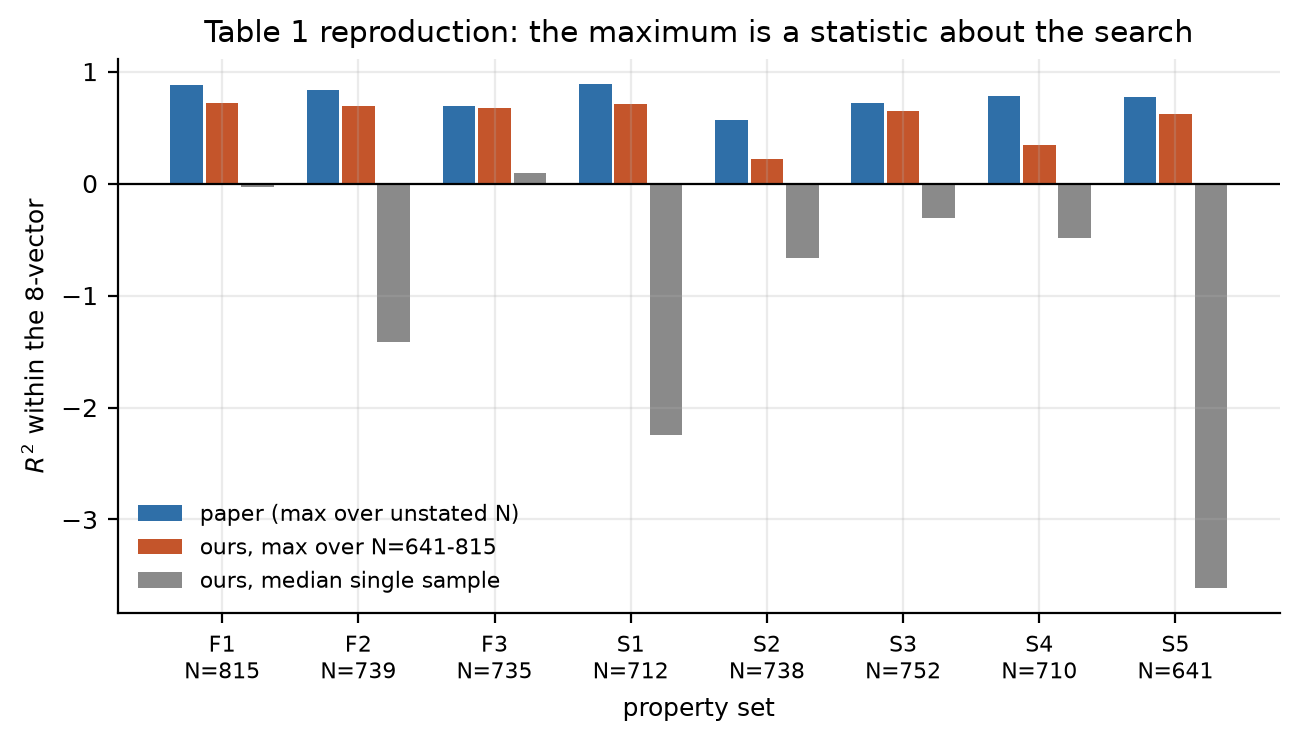
\includegraphics[width=0.92\linewidth]{figures/fig1_table1_reproduction.png}
\caption{Published $R^2$ (left bar of each group), our pool maximum (middle) and
our median single candidate (right), for the eight targets. Tick labels give the
scored pool size for each target. The maxima fall below the published values on
all eight targets; the medians are negative on six.}
\label{fig:table1}
\end{figure}

\begin{figure}[htbp]
\centering
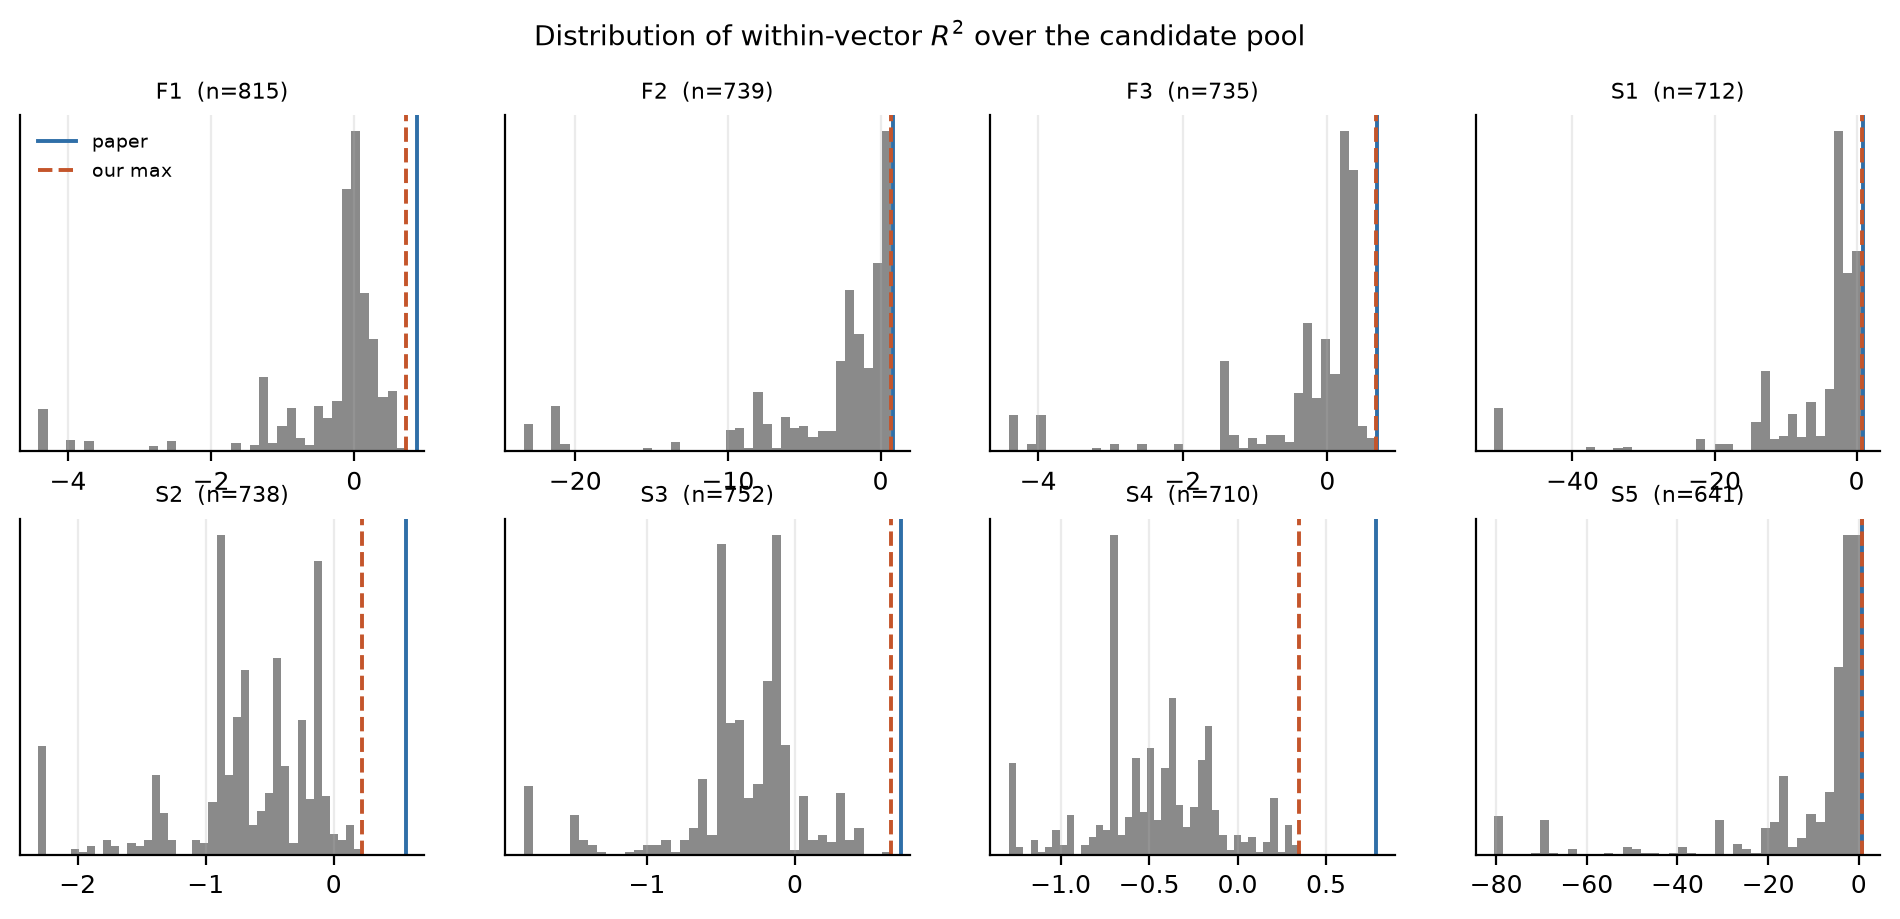
\includegraphics[width=\linewidth]{figures/fig3_r2_distribution.png}
\caption{Distribution of $R^2$ over the scored candidate pool for each target.
Vertical lines mark the published value and our pool maximum. Left tails are
clipped at the second percentile for display; they extend well below the axis
for several targets, which is why the pool means in Table~\ref{tab:table1} are
large and negative.}
\label{fig:r2dist}
\end{figure}

\subsection{Testing whether the decoding choice explains the difference}
\label{sec:gap}

Because the notebook scores candidates with a sampled forward pass, each
candidate's $R^2$ is itself a random variable, and a maximum over noisy scores is
larger than a maximum over noiseless scores. Our forward scores are noiseless.
To test whether this alone accounts for the shortfall, we re-scored the same
candidate sequences with the notebook's sampled forward decoder, changing only
the scorer. The maximum increased by 0.026 on one target and by zero on three
others, a mean of 0.0065, and the scores were identical on 97 to 99\% of
candidates. The greedy decoding choice therefore does not explain a shortfall of
0.27.

\subsection{Submitting the authors' own sequences to the forward task}
\label{sec:exact}

The supplementary material lists the five sequences the authors generated and,
for each, the property vector their forward task predicted. This allows a direct
test of the forward task with a known input and a known expected output.
Table~\ref{tab:exact} gives the result. Four of the five sequences return the
published $R^2$ to four decimal places, and on those four the entire predicted
eight-vector matches the published one entry for entry. The fifth (S2) matches on
six of eight entries and differs on the last two, consistent with the sampled
decoding in the original diverging from greedy decoding on a low-confidence tail.

\begin{table}[htbp]
\centering
\small
\caption{Forward task applied to the authors' own generated sequences. The final
column counts how many of the eight predicted entries match the published vector.}
\label{tab:exact}
\begin{tabular}{lcccc}
\toprule
Target & Length & Published $R^2$ & Our $R^2$ & Entries matching \\
\midrule
S1 & 1096 & 0.8899 & 0.8899 & 8 of 8 \\
S2 & 926 & 0.5640 & 0.5176 & 6 of 8 \\
S3 & 312 & 0.7167 & 0.7167 & 8 of 8 \\
S4 & 869 & 0.7843 & 0.7843 & 8 of 8 \\
S5 & 521 & 0.7751 & 0.7751 & 8 of 8 \\
\bottomrule
\end{tabular}
\end{table}

This result places the shortfall in Section~\ref{sec:table1} in the candidate
search rather than in the forward task, the checkpoint, the prompt format, the
normalisation or the decoding choice. Given the authors' sequences, the forward
task returns the authors' values. The generated sequences reported by the
authors are also longer than the ones our search found (1096, 926, 312, 869 and
521 residues, against 530, 493, 471, 185 and 256 for our best candidates), so the
two searches explored different regions of the sequence space. The reason the
authors' search located longer and higher-scoring candidates cannot be
determined from the available information.

\subsection{Cross-checks against the supplementary tables}

With the authors' sequences available, two further checks were possible. First,
the supplementary material reports molecular weight, instability index and
isoelectric point for all fifteen listed sequences, computed with a standard
tool. Recomputing these gives agreement on 15 of 15 molecular weights, 15 of 15
isoelectric points and 13 of 15 instability indices. The two instability-index
differences occur for the two sequences containing an unknown-residue code; the
tool used by the authors evidently assigned that code an average residue mass of
about 112~Da, which reproduces the published molecular weights exactly, while the
instability index, computed from adjacent residue pairs, is affected by how the
unknown residue is treated.

Second, the motif analysis of the original Figure~7 could be reproduced against
the authors' own comparison sequences using the published motif set. The
correlation between the motif-density profile of each generated sequence and the
mean profile of its two comparison sequences is 0.658, 0.448, 0.941, 0.944 and
0.660 for S1 to S5. This is consistent with the paper's qualitative statement
that the correspondence is strongest for the sets with common and optimised
targets and weakest for set 2.

\section{Extended analyses}

The following analyses were not part of the original paper. They characterise
the behaviour of the released model.

\subsection{Dependence of the reported value on the sampling budget}
\label{sec:bestofn}

The reported $R^2$ is a maximum over a pool of sampled candidates. The size of
that pool is not stated in the paper; the released notebook uses 2{,}048. Because
the maximum of a sample grows with the sample size, the reported value depends on
this budget as well as on the model. Table~\ref{tab:bestofn} gives the expected
maximum as a function of budget, estimated by resampling from each pool, up to a
budget of one tenth of the pool size, beyond which the estimate is dominated by
whether the single largest pool value is drawn. Figure~\ref{fig:bestofn} plots
the same quantity.

\begin{table}[htbp]
\centering
\small
\caption{Expected best $R^2$ after $N$ candidates, estimated by bootstrap
resampling of each pool. The value at $N=1$ is the mean single candidate.}
\label{tab:bestofn}
\begin{tabular}{lccccccc}
\toprule
Target & $N{=}1$ & 2 & 4 & 8 & 16 & 32 & 64 \\
\midrule
F1 & $-0.36$ & $0.06$ & 0.23 & 0.34 & 0.44 & 0.51 & 0.56 \\
F2 & $-3.40$ & $-0.86$ & 0.05 & 0.40 & 0.54 & 0.58 & 0.59 \\
F3 & $-0.34$ & $0.13$ & 0.30 & 0.37 & 0.42 & 0.47 & 0.54 \\
S1 & $-6.49$ & $-2.09$ & $-0.66$ & $-0.07$ & 0.26 & 0.44 & 0.55 \\
S2 & $-0.70$ & $-0.38$ & $-0.22$ & $-0.09$ & $-0.02$ & 0.03 & 0.09 \\
S3 & $-0.36$ & $-0.15$ & $0.01$ & 0.12 & 0.25 & 0.35 & 0.42 \\
S4 & $-0.48$ & $-0.28$ & $-0.10$ & $0.01$ & 0.14 & 0.23 & 0.28 \\
S5 & $-11.71$ & $-3.43$ & $-1.29$ & $-0.45$ & $-0.03$ & 0.21 & 0.34 \\
\bottomrule
\end{tabular}
\end{table}

\begin{figure}[htbp]
\centering

\includegraphics[width=0.82\linewidth]{figures/fig2_bestofn.png}
\caption{Expected best $R^2$ against the number of sampled candidates, on a
logarithmic axis, for the eight targets. Dotted horizontal lines mark the
published values; shaded bands are the 5th to 95th percentiles over bootstrap
replicates. The axis is clipped at $-2$; the single-candidate means for three
targets lie below it.}
\label{fig:bestofn}
\end{figure}

The single-candidate value is negative for six of eight targets, and the curves
rise steeply and monotonically with the budget. The model is unchanged along
each curve. Reporting the budget alongside the maximum, or the curve itself,
would make the number comparable to a single-shot result from another method.

\subsection{Sensitivity of the forward task to sequence content}
\label{sec:ablation}

If the forward task computes properties from sequence features, then editing
those features should change the prediction in an interpretable way. We edited 30
real MaSp sequences in controlled ways and measured the mean absolute change in
the eight predicted values.

Two reference points frame the results. Resubmitting an unedited sequence gives a
change of zero under greedy decoding, so that reference cannot reject any effect.
A single conservative point mutation, one residue replaced by a chemically
similar one, gives a mean change of 0.0148, with a median of zero, and serves as
the smallest meaningful edit. The spread of predictions across different natural
sequences is 0.0874, and effects are reported below as a fraction of this scale.

The main comparison concerns motif knockouts. Removing all poly-alanine tracts,
all GGX repeats or all GPGXX repeats changes both the residues present and the
distribution of the deletion, so each knockout was compared against two
length-matched controls: one that removes the same number of residues at random
scattered positions, and one that removes them as a single contiguous block.
Table~\ref{tab:knockout} gives the result. Every knockout lies between its two
controls. A motif knockout removes several separated runs, so a value between the
scattered and the block control is what removing that number of residues predicts
in the absence of any motif-specific effect. Removing poly-alanine tracts, which
form the crystalline reinforcing blocks, changes the prediction less than
removing the same number of residues at random positions.

\begin{table}[htbp]
\centering
\small
\caption{Motif knockouts against two length-matched controls, as mean absolute
change in the eight-vector prediction. Each knockout lies between its controls.}
\label{tab:knockout}
\begin{tabular}{lccc}
\toprule
Motif & Knockout & Scattered control & Block control \\
\midrule
poly-A & 0.0809 & 0.1043 & 0.0493 \\
GGX & 0.0715 & 0.0914 & 0.0551 \\
GPGXX & 0.0954 & 0.1063 & 0.0429 \\
\bottomrule
\end{tabular}
\end{table}

Figure~\ref{fig:ablation} orders all edits by their effect. Reversing the
sequence (0.132), shuffling it (0.147), block-shuffling it (0.130) and replacing
it with uniform random residues of the same length (0.123) produce changes of
similar size, between 1.4 and 1.7 times the natural-sequence scale. The effect of
an edit therefore saturates: beyond a certain amount of disruption, further
disruption does not move the prediction further. These measurements describe the
model rather than the material. A shuffled or random sequence lies outside the
fine-tuning distribution, so a large change indicates sensitivity to sequence
order without establishing that the model uses order in a mechanically
meaningful way.

\begin{figure}[htbp]
\centering

\includegraphics[width=0.86\linewidth]{figures/fig4_ablation.png}
\caption{Mean absolute change in the forward prediction for each edit, over 30
MaSp sequences. Grey bars are the length-matched controls; the vertical line at
0.087 is the spread of predictions across different natural sequences. The
bottom bar is the single-point-mutation reference at 0.015.}
\label{fig:ablation}
\end{figure}

\subsection{A composition-only baseline}
\label{sec:baseline}

To place the forward task against a simple reference, we fitted ridge regression
and gradient-boosted trees on hand-built features (amino-acid fractions,
dipeptide fractions and motif densities) over the 1{,}033 pairs.
Table~\ref{tab:baseline} gives the mean $R^2$ over the four mechanical
properties, both in-sample and under five-fold cross-validation.
Figure~\ref{fig:baseline} shows the same comparison.

\begin{table}[htbp]
\centering
\small
\caption{Composition-only baselines. In-sample values are fitted and scored on
all 1{,}033 rows; cross-validated values use five folds. Mean $R^2$ over the four
mechanical properties.}
\label{tab:baseline}
\begin{tabular}{llcc}
\toprule
Features & Model & In-sample & 5-fold CV \\
\midrule
composition & ridge & 0.026 & 0.001 \\
composition & gradient boosting & 0.799 & $-0.155$ \\
composition + motifs & gradient boosting & 0.798 & $-0.155$ \\
dipeptide & gradient boosting & 0.870 & $-0.130$ \\
\bottomrule
\end{tabular}
\end{table}

\begin{figure}[htbp]
\centering
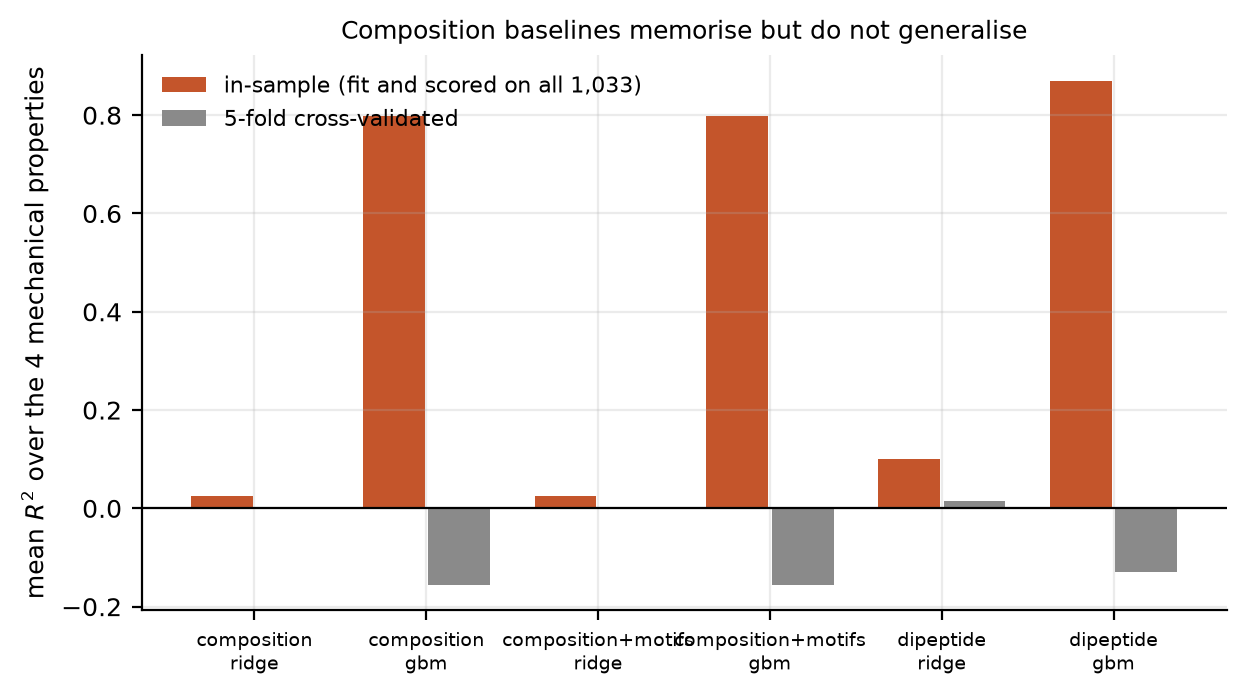
\includegraphics[width=0.82\linewidth]{figures/fig5_baseline.png}
\caption{Composition baselines, mean $R^2$ over the four mechanical properties.
For each feature set and model, the in-sample bar and the cross-validated bar are
shown. The gradient-boosted models fit the training rows well and generalise
below zero.}
\label{fig:baseline}
\end{figure}

The gradient-boosted models reach an in-sample $R^2$ of 0.80 to 0.87 and a
cross-validated $R^2$ below zero. Grouping the cross-validation folds by species,
so that no species appears in both training and test, gives a mean of $-0.049$.
On this dataset, in-sample fit and generalisation are close to unrelated. Because
the paper fine-tunes on all pairs, this observation applies to any in-sample
accuracy measured on those pairs, including the forward-task accuracy in
Section~\ref{sec:memorisation}.

Scored the way the paper scores, as a within-vector $R^2$ per sequence, the
composition ridge baseline reaches a maximum of 0.697 over the 1{,}033 sequences.
This is not a like-for-like comparison with the paper's values, which are maxima
over generated sequences against novel targets, but it shows that a value in the
0.6 to 0.7 range on this metric is reachable without a transformer.

\subsection{Behaviour outside the training family}
\label{sec:nonmasp}

The model was fine-tuned on MaSp only. The dataset contains seven other spidroin
families recovered from the same spiders. Submitting sequences from each family
to the forward task gives the accuracy in Table~\ref{tab:nonmasp} and the mean
predictions in Figure~\ref{fig:nonmasp}. Accuracy is $R^2 = 0.83$ on MaSp and
between $-0.27$ and $-0.54$ on the other families, with the mean absolute error
rising roughly sixfold.

\begin{table}[htbp]
\centering
\small
\caption{Forward-task accuracy by spidroin family, against measured dragline
properties. Only MaSp was in the fine-tuning set.}
\label{tab:nonmasp}
\begin{tabular}{lccc}
\toprule
Family & In training & Mean $R^2$ (mechanical) & Mean absolute error \\
\midrule
MaSp & yes & $0.826$ & 0.024 \\
MiSp & no & $-0.270$ & 0.141 \\
AcSp & no & $-0.317$ & 0.170 \\
AgSp & no & $-0.430$ & 0.158 \\
CySp & no & $-0.472$ & 0.151 \\
Flag & no & $-0.514$ & 0.161 \\
PySp & no & $-0.540$ & 0.152 \\
\bottomrule
\end{tabular}
\end{table}

\begin{figure}[htbp]
\centering
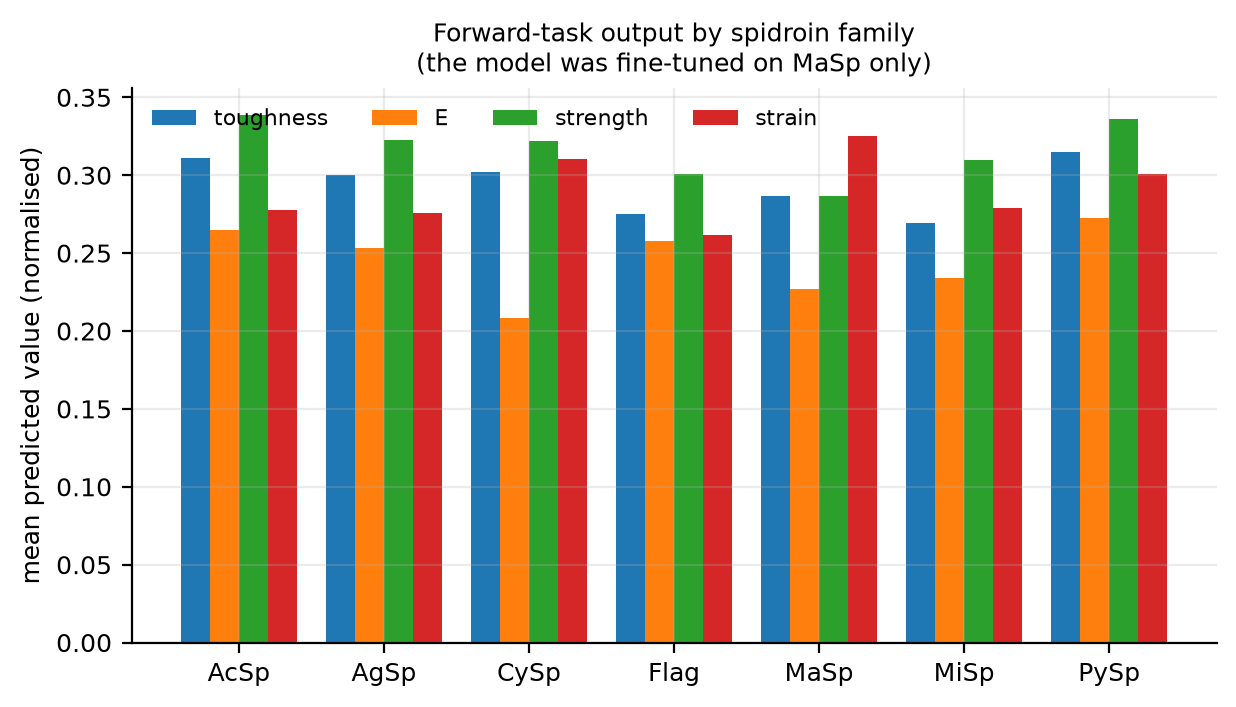
\includegraphics[width=0.82\linewidth]{figures/fig6_nonmasp.png}
\caption{Mean predicted value for each of the four mechanical properties, by
spidroin family. The heights are similar across families despite large
differences in the underlying proteins.}
\label{fig:nonmasp}
\end{figure}

The predictions also vary little with family. The between-family spread of the
mean prediction is 0.019, against a within-family spread of 0.095, both over the
four mechanical properties, a ratio of 0.199. Given a sequence it has not
memorised, the model returns a value close to its training marginal regardless of
family. One caveat applies to the accuracy column but not to the spread ratio:
the mechanical properties describe dragline, so a non-MaSp sequence is paired
with its spider's dragline properties rather than with the properties of its own
silk type. The accuracy column therefore measures recovery of dragline properties
from a non-MaSp sequence, not prediction of that sequence's own silk.

\subsection{In-sample forward accuracy and label reproduction}
\label{sec:memorisation}

Over the 1{,}033 pairs, the forward task reaches a mean in-sample $R^2$ of 0.696
across the four mechanical properties (Table~\ref{tab:forward}). Of the 1{,}026
sequences that parsed, 732, or 71.3\%, return all eight values within 0.0005 of
the training label, which is the resolution the model prints. The mean absolute
error on those sequences is 0.00025. On the remaining 294 sequences the mean
absolute error is 0.109 and the mean $R^2$ over the four mechanical properties is
$-0.113$.

\begin{table}[htbp]
\centering
\small
\caption{In-sample forward accuracy per property over the 1{,}033 pairs.}
\label{tab:forward}
\begin{tabular}{lccc}
\toprule
Property & In-sample $R^2$ & Pearson $r$ & Mean absolute error \\
\midrule
toughness & 0.806 & 0.900 & 0.022 \\
toughness SD & 0.741 & 0.867 & 0.033 \\
$E$ & 0.578 & 0.791 & 0.028 \\
$E$ SD & 0.389 & 0.739 & 0.037 \\
strength & 0.721 & 0.854 & 0.029 \\
strength SD & 0.566 & 0.777 & 0.039 \\
strain & 0.681 & 0.838 & 0.027 \\
strain SD & 0.644 & 0.823 & 0.036 \\
\bottomrule
\end{tabular}
\end{table}

The in-sample $R^2$ therefore rests substantially on sequences whose label is
reproduced exactly, and is negative on the remainder. The value of $-0.113$ is
not a generalisation estimate: those sequences are selected by outcome and differ
from the rest, with a median length of 456 against 361 residues, so the
selection biases the estimate downward by an unknown amount. Obtaining a
generalisation estimate would require retraining with a held-out fold, which was
not done here.

In the inverse direction, the same pattern appears. Across the eight targets,
62.3\% of parsed generations are exact copies of sequences in the reference set;
these span 200 to 290 distinct known sequences per target. The default behaviour
of the inverse task therefore includes a large fraction of retrieval, which is
why the scored pools in Table~\ref{tab:table1} are well below the generation
budget. This does not affect the paper's reported results, which are computed
only over the novel generations, but it does describe how the model behaves
before that filter is applied.

\section{Notes on the paper and corrections to our own work}

Several points arose that are recorded for completeness.

The secondary-structure fractions in the original Figure~5 are defined in its
caption using the amino-acid groupings that a common analysis library used up to
version 1.81. That library corrected the groupings in version 1.82, noting that
the earlier version returned the sheet and helix labels transposed. Under the
corrected grouping, the labels in that figure are exchanged. The paper used the
library as documented at the time. We compute both conventions and report both,
since beta-sheet content is central to silk mechanics.

The value of strength for target S3 is given as 0.200 in both Table~1 and the
Figure~2 caption of the paper, while the stated rule sets non-varied properties
to the dataset median, which is 0.310 for strength as used in S1, S2 and S4. We
kept the published value, since changing a published input to improve agreement
would not be a reproduction. This affects the target spread and therefore the
$R^2$ for S3.

Three claims we made during this work were incorrect and were subsequently
withdrawn, and we record them because the cause is instructive. We first reported
that three entries in the paper's motif table carried the opposite sign to the
source they cite; this was an error introduced by reading a two-column table
from linearised text, in which the two columns interleaved, and all fourteen
entries in fact agree with the source. We first extracted the authors' generated
sequences with an error that misassigned one line of text per affected row; the
sequence lengths still matched the published lengths, because every line has the
same width, and the error was found only by checking the published molecular
weights, which depend on residue identity. We first reported that a
composition-difference analysis recovered 12 of 14 published residues; a
permutation test showed that the selection rule recovers about the same number
from random data, so the result was not distinguishable from chance and the
corrected analysis reports a null result. In each case the error survived
internal checks and was caught only by comparison against an independent
published quantity.

\section{Discussion}

The parts of the paper that can be checked directly are reproduced. The released
checkpoint matches the stated architecture and parameter count, it returns the
published property vector for the published worked example, the dataset
reconstructs to the exact published count, and the normalisation constants match
the published table. Given the authors' own generated sequences, the forward
task returns the published $R^2$ to four decimal places on four of five sets,
with the full predicted vector matching entry for entry.

The design procedure reproduces partially. Running it end to end with the
reported budget, our best selected candidate is below the published value on all
eight targets. Since the forward task reproduces exactly on the authors'
sequences, the difference lies in the inverse search rather than in the scorer
or the model. Our search did not find candidates as strong as the authors',
and the reason is not recoverable from the available information.

The extended analyses describe what the reported numbers measure. The value is a
maximum over a sampling budget that is not stated, of a within-vector
self-consistency measure, from a model that returns the exact training label for
71\% of its fine-tuning sequences and copies a training sequence in 62\% of
generations. None of this contradicts the paper, which states that it trains on
all pairs and reports self-consistency rather than held-out accuracy. The
observations do indicate that the reported number should be read narrowly. A
self-consistency value from a model that has largely reproduced its training set
is weaker evidence of a learned sequence-property map than the same number from a
model evaluated on held-out data, and the two cannot be distinguished from the
reported figures alone.

Two changes would remove most of this ambiguity and require no new experiments:
stating the sampling budget alongside any selected maximum, and holding out a
fold of the data for evaluation. On 1{,}033 pairs a held-out fold is inexpensive,
and the baseline comparison suggests it would be informative, since in-sample and
cross-validated performance on this data differ by the gap between 0.80 and
$-0.16$.

\subsection*{Limitations}

This work uses the released model and does not retrain it, so it cannot report a
held-out accuracy for SilkomeGPT. The novelty analysis of the original paper
relies on sequence-alignment searches that were not run here; offline
composition-based measures were used as substitutes and are labelled as such. The
structural comparison using folding prediction was not attempted. The ablation
results describe the model's response to sequence edits and are not statements
about the mechanical behaviour of real silk. None of the generated sequences were
synthesised or tested.

\section{Conclusion}

The reproducible components of the paper reproduce, in several cases exactly. The
reported design-procedure values reproduce partially, with the difference
attributable to the candidate search rather than the model. The reported
self-consistency values are maxima over an unstated sampling budget from a model
that reproduces much of its training set in both task directions, and are best
read as self-consistency of a largely retrieval-based system rather than as
evidence of a generalising sequence-property map. Reporting the sampling budget
and evaluating on held-out data would resolve the remaining ambiguity.

\section*{Data and code availability}

The analysis code, the reconstructed dataset builder, and per-run manifests
recording software versions, seeds and the model revision are in the
accompanying repository. The model checkpoint and the Silkome primary data are
available from their original sources and are not redistributed here.

\begin{thebibliography}{9}
\small
\bibitem{lu2024} W. Lu, D. L. Kaplan, M. J. Buehler. Generative Modeling,
Design, and Analysis of Spider Silk Protein Sequences for Enhanced Mechanical
Properties. \textit{Advanced Functional Materials} \textbf{34}, 2311324 (2024).
Preprint: arXiv:2309.10170.
\bibitem{arakawa2022} K. Arakawa et al. 1000 spider silkomes: linking sequences
to silk physical properties. \textit{Science Advances} \textbf{8}, eabo6043
(2022).
\end{thebibliography}

\end{document}
